
\chapter{Automatic Detection of InSAR Surface Deformation Signals In the Presence Severe Tropospheric Noise}

%In this chapter, we demonstrate methods for automatically detecting surface deformation signals in InSAR maps. We present a computer vision algorithm based on Laplacian of Gaussian filters. We show how the tropospheric noise levels can be estimated from InSAR data, and we use these estimates to simulate new instances of noise. We create confidence measures based on the simulations for automatically detected signals in real InSAR maps.


\section{Introduction}
\label{sec:ch6-intro}

Detection of surface deformation signals in maps derived from interferometric synthetic aperture radar (InSAR) poses a challenge due to the ubiquity of spatially correlated tropospheric turbulence noise. In this chapter,
we combine methods for tropospheric noise characterization with computer vision algorithms for detecting surface deformation.
We first present our computer vision algorithm, based on Laplacian of Gaussian (LoG) filtering, for finding signals of unknown size and location within InSAR deformation maps.
LoG-based detection algorithms were developed in the computer vision literature to detect repeatable image feature points at many scales \citep{Witkin1987ScaleSpaceFiltering, Lindeberg1998FeatureDetectionAutomatic}, and gained widespread use through the success of the Scale Invariant Feature Transform (SIFT) algorithm \citep{Lowe2004DistinctiveImageFeatures}. 
% for detecting surface deformation signals of unknown location and size in InSAR deformation maps. 
Additionally, we estimate expected magnitude of tropospheric artifacts in InSAR deformation maps by calculating the power spectral density of our study region's tropospheric noise and simulating many instances of similar noise.
We combine these two techniques to derive an empirical probability density function (PDF) of the size and magnitude of noise artifacts in our study region.
We demonstrate the performance of the algorithm on the two paths of Sentinel-1 data from Chapter \ref{CHAP:4-GRL} acquired between 2014 and 2019 over the oil-producing Permian Basin in West Texas. 
Several hundred deformation features are identified in areas known to contain clusters of oil production, wastewater injection, and seismic activity. 
%The algorithm detects many more features in both paths over time as 
%well on both paths of data, despite large variations in the strength of tropospheric noise between
We note that our algorithm detects surface deformation features caused by a wide variety of anthropogenic and natural causes despite requiring no prior physical models of the features of interest. Additionally, we generate confidences for each detected visual feature. Although we demonstrate the detection algorithm on cumulative deformation maps derived from stacking interferograms, it can be easily adapted to other types of multi-temporal InSAR time series methods.



%\section{Review of Automatic Deformation Detection for InSAR}

%With the launch of Sentinel-1, acquiring 250-km wide swaths of data every 6-12 days, several groups developed automated processing chains for producing regional or global databases of surface deformation using short-baseline interferograms.
%Several of these were applied to monitor volcano deformation \citep{Meyer2015IntegratingSarDerived, Valade2019TowardsGlobalVolcano, Lazecky2020LicsarAutomaticInsar}.
%Due to the large quantity of data, the early automatic detectors used pixel-wise metrics, such as changes to coherence \citep{Meyer2015IntegratingSarDerived}, thresholds on deformation velocity \citep{Raspini2018ContinuousSemiAutomatic, Bekaert2020InsarBasedDetection} or receiver operating characteristic cumulative sum control charts \citep{Albino2020AutomatedMethodsDetecting}. Other pixel-wise approaches have processed individual time series using dimensionality reduction or feature mapping mapping techniques, such as t-SNE \citep{Kerkhof2020IndividualScattererModel} or Long Short-term Memory Autoencoders (LSTM-AE) \citep{Ansari2021InsarDisplacementTime}, followed by density-based clustering algorithms.
%
%Classical machine learning approaches, such as principal component analysis (PCA) or independent component analysis (ICA), have also been exploited to separate deformation signal from noise \citep{Chaussard2014PredictabilityHydraulicHead, Ebmeier2016ApplicationIndependentComponent, Gaddes2018BlindSignalSeparation}. 
%These signal separation techniques may take entire deformation images as input, or may be performed pixel-wise on time series to cluster anomalous behaviors.
%Deep learning approaches using convolutional neural networks (CNNs) have been applied to automatically detect and localize features in InSAR deformation maps \citep{Anantrasirichai2018ApplicationMachineLearning, Anantrasirichai2019ApplicationConvolutionalNeural, Anantrasirichai2019DeepLearningApproach, Anantrasirichai2021DetectingGroundDeformation}.
%These efforts used large pretrained models, such as AlexNet \citep{Krizhevsky2012ImagenetClassificationDeep} or VGG19 \citep{Simonyan2014VeryDeepConvolutional}, that were adapted from RGB image classification benchmarks; this necessitated a pre-processing step of re-wrapping and/or colorizing the deformation maps to feed into the 3-channel RGB input. The models in \citep{Anantrasirichai2019DeepLearningApproach} were trained using labeled input data that was synthetically generated using noise and deformation models, in addition to the labeled real data from \citep{Anantrasirichai2018ApplicationMachineLearning}.
%CNN models were trained from scratch on synthetis data in \citep{Valade2019TowardsGlobalVolcano}
%to learn a decorrelation mask from input wrapped interferograms and detect volcanic ground deformation.  The authors in \citep{RouetLeduc2021AutonomousExtractionMillimeter} created a denoising autoencoder \citep{Vincent2008ExtractingComposingRobust}, also trained on synthetically generated data, which ingested 9 noisy patches of deformation time series maps and detected transient deformation based on an Okada fault model \citep{Okada1992InternalDeformationDue} or inflation/deflation from a Mogi point-source model \citep{Mogi1958RelationsEruptionsVarious}.
%
%
%Separate from the machine learning and computer vision work, several efforts have analyzed atmospheric noise levels in an attempt to yield a minimum-detectable deformation threshold.
%The earliest case of this was \citep{Emardson2003NeutralAtmosphericDelay}, who calculated an expected number of acquisitions needed to reliably detect some linear velocity given an atmospheric noise level $\sigma$. This work was extended to use external data sources.
%A Monte Carlo technique for generating pseudo-InSAR time series was developed in \citep{Barnhart2013CharacterizingEstimatingNoise}, which used sets of MODIS data over the same temporal range as the available SAR imagery.
%\citep{Parker2015SystematicAssessmentAtmospheric} used the North American Regional Reanalysis (NARR) weather model to produce estimates of atmospheric noise variance $\sigma$ on each SAR acquisition; similar to \citep{Emardson2003NeutralAtmosphericDelay}, these were propagated through a weighted least squares inversion to produce a pixel-wise uncertainty level on deformation velocities. \citep{Havazli2021DetectionThresholdEstimates} computes minimum deformation velocity thresholds based on the simulation of stratified and turbulent tropospheric noise. The authors simulate noise without deformation and compute expected ranges of residual tropospheric noise. The authors of, \citep{Havazli2021DetectionThresholdEstimates} that different study areas have different noise parameters, but do not present a way to estimate these noise levels directly from InSAR data, instead relying using MODIS PWV data to obtain a multiplier parameter for the strength of the stratified noise.
%




\section{Methods}
\label{sec:methods}


\subsection{Automatic Feature Detection}
\label{subsec:methods-1-log}

Given a surface deformation map $M$ derived from InSAR data, the value $ M_{ij} $ at the $i^{th}$ row and $j^{th}$ column represents the magnitude of a cumulative, seasonal, or transient deformation signal at this pixel. Because the earth can be considered as a stratified elastic-viscoelastic medium, surface deformation features are often spatially coherent \citep{Segall2010EarthquakeVolcanoDeformation}. In this study, our goal is to automatically detect these features in an InSAR deformation map $M$ that covers a very large region (Algorithm 1).

There have been many computer vision algorithms that were designed to automatically detect spatially coherent ``blob-like'' features in 2D image data \citep{Lindeberg1993DetectingSalientBlob, Lindeberg1998FeatureDetectionAutomatic, Lowe2004DistinctiveImageFeatures}. In this study, we employ the Laplacian of Gaussian (LoG) filters as a blob detector. An LoG kernel $K^{(m)}$ with a size $\sigma_m$ is written as:
\begin{equation}
	K^{(m)}_{ij} = \left(\frac{(i - l)^2 + (j - l)^2 - 2\sigma_m^2}{2 \pi \sigma_m^4}\right) \, e^{-\frac{ (i - l)^2 + (j - l)^2}{2 \sigma_m^2}} \label{eq:log-kernel}
\end{equation}
where pixel indices $ij  \in \left\lbrace 0, 1, \ldots, 2l \right\rbrace$. The unit of $\sigma_m$ is given in pixels, which can be scaled to meters based on the pixel spacing of the InSAR deformation map $M$.


We generate a set of LoG kernels $K^{(1)}, K^{(2)}, \ldots$ with progressively larger $\sigma_m$ (Figure \ref{fig:log-kernel}), and calculate the $m^{th}$ filter response $ L^{(m)} $ as:
\begin{equation}
	L^{(m)} = M \ast K^{(m)}  \label{eq:log-layer-conv}
\end{equation}
Here $*$ denotes the 2D discrete convolution, which is typically computed using the Fast Fourier Transform (FFT) algorithm because of its superior computational efficiency \citep{Szeliski2022ComputerVision}.


\begin{figure}[hbt!]
	\centering
	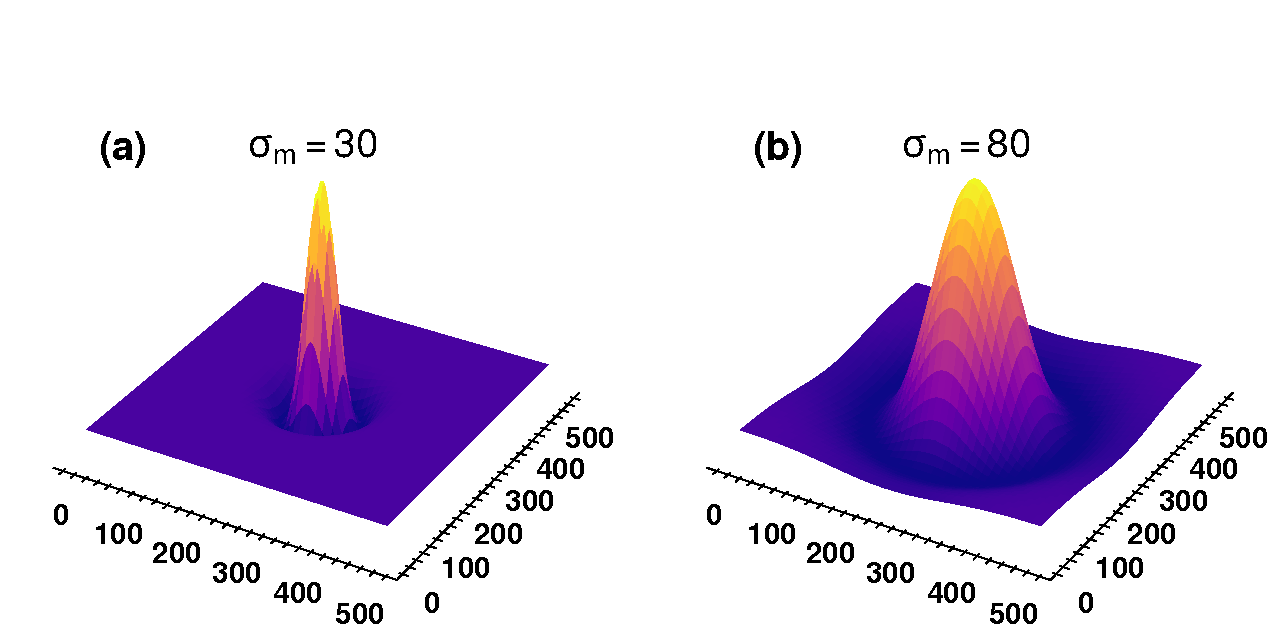
\includegraphics[width=0.98\linewidth]{paper2/figures/figure1_log_examples.pdf}
	\caption[Laplacian of Gaussian (LoG) kernels]{
		Laplacian of Gaussian (LoG) kernels with (a) $\sigma_m=30$ pixels and (b) $\sigma_m=80$ pixels for an image of size of 500-by-500 pixels.
	}
	\label{fig:log-kernel}
	%
\end{figure}

To demonstrate how to estimate the size of an unknown deformation feature from the filter responses, Figure \ref{fig:log-response} (a) shows a $500 \times 500$ synthetic deformation map $M$ that contains one Gaussian-shaped uplift feature in the upper left and one elliptical Gaussian subsidence feature in the lower right. We filtered this deformation map using 20 LoG kernels of sizes ranging from $\sigma_1 = 3$ pixels to $\sigma_{20} = 100$ pixels with a base-2 logarithmic spacing, and the filter responses are shown in Figure \ref{fig:log-response} (b)-(e). For the round uplift case, the filter response $L^{(m)}$ (the black curve in Figure \ref{fig:log-response} (b)) is strongest when the kernel size $\sigma_m$ matches the deformation feature radius $r$ as $r = \sqrt{2}\sigma_m$. This is known as the extreme point, or the local maximum points of $|L^{(m)}|$ for all attempted $\sigma_m$. For the elliptical subsidence case, the extreme point is reached when the average length of the two primary axes of the deformation feature is $\sim \sqrt{2}\sigma_m$ (the green curve in Figure \ref{fig:log-response} (b)). For the case of no deformation, no substantial filter response is generated for any filter size (the gold curve in Figure \ref{fig:log-response} (b)).



\begin{figure}[hbt!]
	\centering
	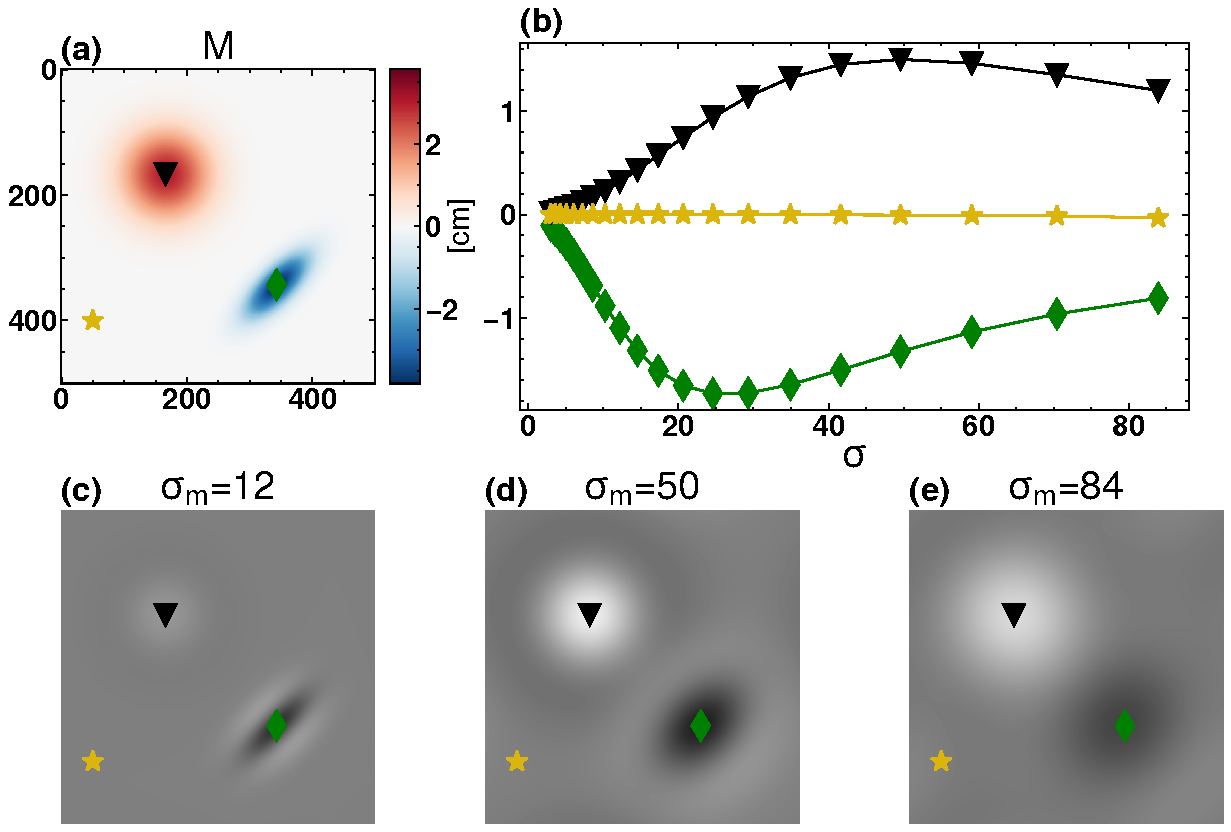
\includegraphics[width=0.98\linewidth]{paper2/figures/figure2_log_response.pdf}
	\caption[LoG filter responses to synthetic deformation]{
		(a) A synthetic deformation map that contains one Gaussian-shaped uplift feature in the upper left and one elliptical Gaussian subsidence feature in the lower right. (b) LoG response amplitudes for 20 filters with various sizes ($\sigma_m$) at three marker points. The marker locations are shown in panel (a). (c)-(e) The LoG filter responses for $\sigma_m=$ 12, 50, and 84.}
	\label{fig:log-response}
	%
\end{figure}

In the case that two candidate blobs have more than 50\% overlapping area, the blob with a smaller size is discarded. 
Additionally, the LoG filter may falsely flag ghost blobs at the edges of real deformation features. This is because deformation features with strong curvature at the center also contain a strong opposite-signed curvature near the border \citep{Lindeberg1998FeatureDetectionAutomatic}. To remove those false positives, we use the distance from the candidate blob's center location to the nearest deformation amplitude extremum as a measure. If this distance is close to the blob radius, the detection is likely a ghost blob. In our test case, we discarded blobs with local extremum distances larger than 75$\%$ of the blob radius, which effectively removed all visible false positives near the edge of real deformation features.

For the $k^{th}$ detected deformation feature, our algorithm outputs the blob center location $(i_k, j_k)$, the blob radius $ r_k$, the filter response magnitude $|g_k|$ at the extreme point, and the deformation magnitude $|\bar{d_k}|$ defined as the weighed maximum of all pixels within the $k^{th}$ blob:
\begin{equation}
	\bar{d_k} = \max_{kk} |w_{kk} M_{kk} | 
\end{equation}
Here the weight $w_{kk}$ equals $\exp\left[-(r_{kk} / r_k)^2\right]$, where $r_{kk}$ is the distance between a pixel within the blob and the blob center. The exponential weighting prevents pixel outliers from distorting the measure of feature magnitude. 

We can exclude undesired deformation features by setting magnitude thresholds on $|g_k|$ and $|\bar{d_k}|$ based on users' interest. Furthermore, we need to determine whether a detected deformation feature has a signal magnitude above the noise level of the InSAR deformation map, which is the focus of the following method sections. 


\begin{algorithm}
	\caption{LoG Based Deformation Feature Detection}\label{algo:blobs}
	\SetAlgoLined
	\KwIn{2D InSAR deformation map $M$}
	\KwResult{For each $k \in {1, \ldots, N_d}$ detections, the algorithm outputs the blob center location $ (i_k,j_k) $, the blob radius $ r_k $, the filter response magnitude $|g_k|$ at the extreme point, the deformation magnitude $|\bar{d_k}|$ }
	
	// Calculate filter responses:\\
	\ForEach{$ \sigma_m \in \left\lbrace \sigma_{min} \ldots \sigma_{max}\right\rbrace $}{
		%$L^{(n)} = \mathcal{F}^{-1} \left[ \mathcal{F} M \cdot  \mathcal{F} K^{(n)} \right] $
		$ L^{(m)} = M \ast K^{(m)}  $
		%$\nabla^2_{norm} L(\cdot, \cdot, \sigma) \gets I(\cdot, \cdot) * \nabla^2_{norm} G(\cdot,\cdot, \sigma)$
	}	
	// Find candidate blobs from local extrema:\\
	\For{$ (i, j, m) \in  L $}{
		\If{$L[i, j, m] $ is local extremum }{
			% \If{$\det \mathcal{H}_{norm} L(x,y,\sigma ) $ is local extremum }{
				Compute $ r = \sqrt{2}\sigma_m $ \\
				Add $ (i, j, r) $ to list of candidate detections
			}
		}
		// Prune blobs with overlap:\\
		\ForEach{$ b_1 := (i_1, j_1, r_1), b2 := (i_2, j_2, r_2) \in $ candidates}{
			%	Form circle of radius $ r_i $ around $ (i_1, j_1) $\\
			\If{ Overlap$( b_1, b_2 ) > 0.5 $  }{
				Remove smaller of $ b_1, b_2 $
			}
		}
		
		// Prune edge blob false positives:\\
		\ForEach{$ b_k := (i_k, j_k, \sigma_k) \in $ candidates}{
			Find coordinates $(u, v)$ of local max of $M$ within
			radius $r_k$ around $ (i_k, j_k) $
			\\
			\If{ $\sqrt{(x - u)^2 + (y - v)^2} > 0.75 $  }{
				Discard $ b_k $
			}
		}
		// Prune with thresholds $ \gamma_g, \gamma_d $:\\
		\ForEach{$ b_k := (i_k, j_k, r_k,|g_k|, |\bar{d_k}|) \in $ candidates}{
			\If{ $ |g_k| <  \gamma_g $ \text{or} $ |\bar{d_k}| <  \gamma_d $  }{
				Discard $ b_k $
			}
		}
	\end{algorithm}
	
	
	
\subsection{Tropospheric Noise Spectrum}
\label{subsec:methods-2-tropo-spectrum}
InSAR measurement noise can produce spatially coherent "blob-like" features that are detectable by our algorithm.  Here we focus on characterizing the tropospheric turbulence noise in each SAR scene. This is because tropospheric turbulent noise (1) is correlated in space \citep{Emardson2003NeutralAtmosphericDelay, Lohman2005SomeThoughtsUse}; (2) is present in all InSAR data sets with greatly varying magnitudes \citep{Barnhart2013CharacterizingEstimatingNoise, Hooper2012RecentAdvancesSar}; and (3) is often the primary noise source that limits InSAR measurement accuracy \citep{Jolivet2014ImprovingInsarGeodesy, Bekaert2015StatisticalComparisonInsar, Parker2015SystematicAssessmentAtmospheric}.


Consider an interferogram formed using two SAR scenes acquired at times $t_1$ and $t_2$. In the case that tropospheric turbulence noise is the dominant noise term, the measured interferometric phase $\phi_{1,2}$ (in radians) at a pixel of interest can be written as \citep{Zebker1997AtmosphericEffectsInterferometric}:
\begin{equation}
	\phi_{1,2} \approx \frac{4 \pi}{\lambda} \left(\alpha_2 - \alpha_1 + \Delta d_{1,2} \right)
\end{equation}
where $ \lambda $ is the radar wavelength, $\alpha_1$ and $\alpha_2$ represent the tropospheric delay at the two SAR acquisition times $t_1$ and $t_2$, and $\Delta d_{1,2} $ is the Line-Of-Sight (LOS) deformation ($d_2-d_1$) between $t_1$ and $t_2$. The unit of $\lambda$, $\alpha_1$, $\alpha_2$, and $\Delta d_{1,2} $ is in centimeters. 

Given $N$ SAR acquisitions, we can estimate the tropospheric noise on the $n^{th}$ SAR acquisition date by averaging $N-1$ interferograms that share the common reference SAR scene $n$ \citep{Tymofyeyeva2015MitigationAtmosphericPhase}:
\begin{equation}
	\bar{\alpha}_n = \frac{\lambda}{4 \pi} \frac{1}{N-1} \left(\sum_{k=1, k \neq n}^{N} \phi_{k,n}\right)  =  \alpha_n  + \frac{1}{N-1} \left( \sum_{k=1, k \neq n}^{N}  \Delta d_{k,n} - \sum_{k=1, k \neq n}^{N}  \alpha_k  \right)  \label{eq:avg-ifg} 
\end{equation}
%Note that the interferograms are all formed with $k$ as the reference date; any interferogram which was processed using $k$ as the secondary is multiplied by $-1$ before averaging. 
Because tropospheric turbulence noise is uncorrelated in time for scales longer than one day \citep{Emardson2003NeutralAtmosphericDelay, Onn2006ModelingWaterVapor}, the term $ \frac{1}{N-1} \sum \alpha_k \rightarrow 0$ when  when $N$ is sufficiently large. 
Under the assumption that $ \frac{1}{N-1} \sum \Delta d_{k,n} $ is relatively small comparing to $\alpha_n$, we compute $ \bar{\alpha}_n $ at each pixel to obtain a tropospheric turbulence noise map $A^{(n)}$ for the $n^{th}$ SAR acquisition date over the entire study area. In Section \ref{sec:results:path78}, we further discuss the impact of the deformation signals on our tropospheric noise analysis.


We next compute the 2D Power Spectral Density (PSD) of the $n^{th}$ tropospheric noise estimates at  wavenumber $ k_x, k_y $ (with units $1/m$) as \citep{Jacobs2017QuantitativeCharacterizationSurface}:
\begin{equation}
	\text{PSD}_n(k_x, k_y) = \frac{| \widehat{A^{(n)}} |^2 }{N_x N_y (\frac{1}{\Delta x \Delta y}) } \label{eq:pow-spec}
\end{equation}
where  $\widehat{A^{(n)}}$ is the Discrete Fourier transform (DFT) of  the $n^{th}$ tropospheric noise map $A^{(n)}$, $\Delta x$ and $\Delta y$ are the interferogram pixel spacings (in meters) in the $x$ and $y$ directions, $N_x$ and $N_y$ are the total number of pixels in the $x$ and $y$ directions, and the squared absolute value and division are pixel-wise operations. 


As an example, Figure \ref{fig:psd-example} (a) shows a synthetic 2D tropospheric turbulence noise map. We calculate the 2D PSD of the noise map following Equation \eqref{eq:pow-spec} (Figure \ref{fig:psd-example} (b)). Under the assumption that tropospheric noise is isotropic, we average all pixels with a distance  $k= \sqrt{k_x^2 + k_y^2}$ from the origin to generate a 1D PSD as a function of $k$ \citep{Hanssen2001RadarInterferometryData}.
We plot the 1D PSD on a log-log scale, which rolls off following a power law at higher frequencies (Figure \ref{fig:psd-example} (c)). By contrast, the power spectrum of spatially uncorrelated while noise is relatively flat across all frequencies $k$ (Figure \ref{fig:psd-example} (d)-(f)).




\begin{figure}
	\centering 
	%\includegraphics[width=0.98\linewidth]{figures/figure3_psd_radial.pdf}
	\includegraphics[width=0.98\linewidth]{paper2/figures/figure3_psd_radial.png}
	\caption[Example 1D tropospheric PSD estimation]{
		(a) A simulated 2D turbulent atmospheric noise map with $ 500 \times 500 $ pixels at $100$ meter pixel spacing.
		(b) 2D Power Spectral Density (PSD) of the tropospheric noise map in panel (a).
		(c) 1D PSD as a function of wavenumber $k = \sqrt{k_x^2 + k_y^2}$, under the assumption that tropospheric noise is isotropic.
		(d) A simulated 2D white noise map (spatially uncorrelated) with the same dimension and pixel spacing as panel (a)
		(e) 2D PSD of the white noise map in panel (d).
		(f) 1D PSD as as a function of wavenumber $k = \sqrt{k_x^2 + k_y^2}$. Here We averaged the 1D PSD of 50 2D white noise instances to improve the statistical stability of the spectral estimates.
	}
	\label{fig:psd-example}
\end{figure}


\subsection{Uncertainty Quantification}
\label{subsec:methods-3-noise-sim}

Using the average 1D PSD of all $N$ InSAR-observed tropospheric turbulence noise maps, we can simulate $N$ 2D noise incidences  $S^{(1)},\dots, S^{(N)} $ that closely resemble the real tropospheric noise over the study area \citep{Hanssen2001RadarInterferometryData}. Using these simulated noise maps, we form up to $N(N-1)/2$ noise-only interferograms, and derive a time series solution following the same method for generating the real InSAR deformation map $M$ (e.g. \citep{Sandwell1998PhaseGradientApproach, Berardino2002NewAlgorithmSurface}). Because these synthetic interferograms contain no deformation, any "blob-like" features in the simulated time series solution are associated with tropospheric noise. We record the radius $r_k$,  the filter response magnitude $|g_k|$ and the magnitude $|\bar{d_k}|$ of each noise feature using our automatic blob detection algorithm.

Similarly, we generate many synthetic InSAR data sets that share the same noise spectrum derived from data, and record all detected noise blobs. We create 2D histograms of the noise attributes (filter response magnitude vs. radius and deformation magnitude vs. radius), which allows us to remove candidate blob features in the real deformation map $M$ that are likely due to tropospheric noise artifacts.

\section{Test Site and Available InSAR Data}
\label{sec:site}

We tested our deformation detection algorithm on over an 80,000 $km^2$ oil-producing region in the Permian Basin, West Texas.  As described in \citep{Staniewicz2020InsarRevealsComplex}, we processed 84 ascending Sentinel-1 scenes (Path 78, Frames 94–104) acquired between November 2014 and January 2019 (Figure \ref{fig:study-area}). We imposed no maximum spatial baseline and a maximum temporal baseline of 800 days for interferogram selection, resulting in 2550 multi-looked interferograms with 120 m pixel spacing.  We used the GPS station TXKM as the reference location, where little surface deformation was observed over the study period (Figure \ref{fig:study-area}, yellow dot).

%\begin{figure}[hbt!]
%	\centering
%	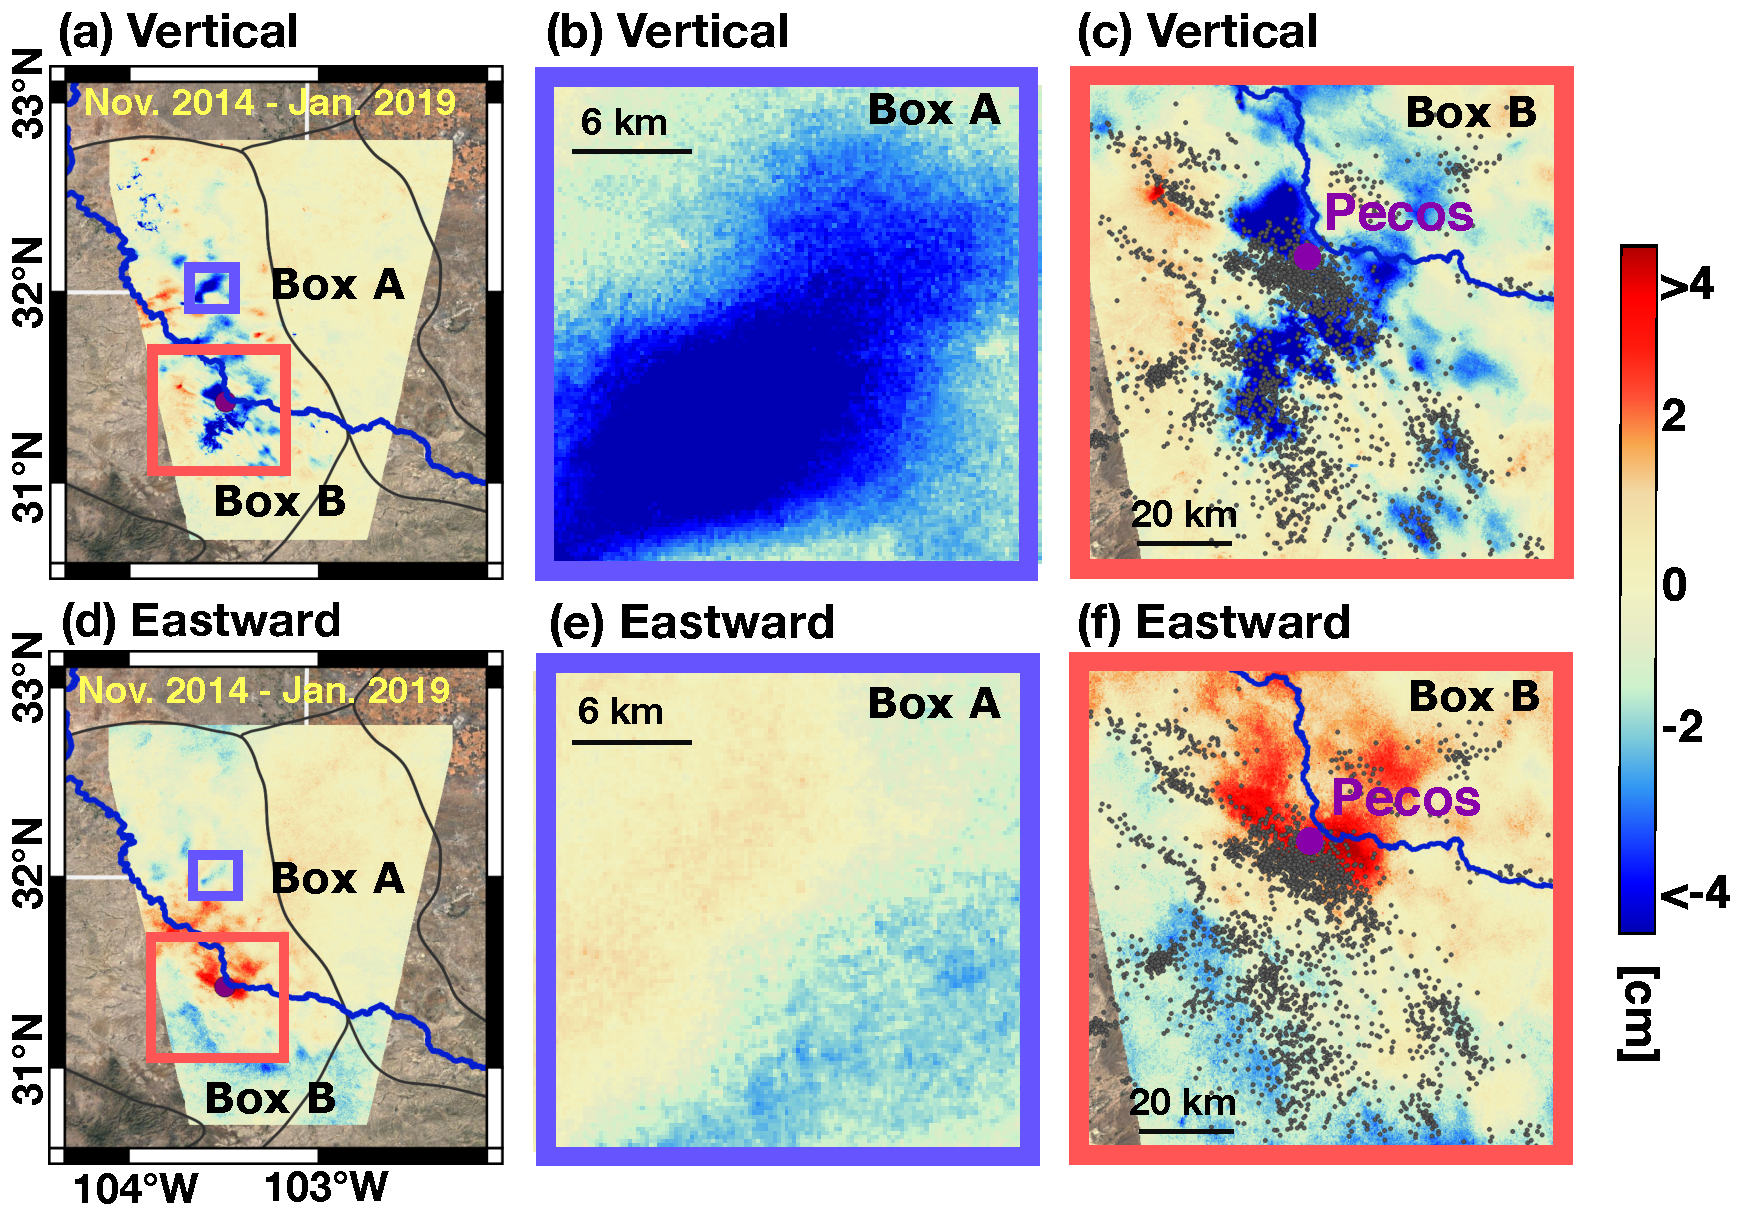
\includegraphics[width=0.96\linewidth]{paper1-permian/figures/figure4-east-vertical-6panel-labelled.pdf}
%	\caption[Cumulative vertical and horizontal deformation]{(a) Cumulative vertical deformation between Nov. 2014 and Jan. 2019 over the region where Sentinel-1 path 78 and path 85 overlap. A zoomed-in view of Box A in the northern Delaware Basin and Box B in the southern Delaware Basin are shown in panel (b) and (c) respectively. (d) Cumulative eastward deformation between Nov. 2014 and Jan. 2019 over the region where Sentinel-1 path 78 and path 85 overlap. A zoomed-in view of Box A in the northern Delaware Basin and Box B in the southern Delaware Basin are shown in panel (e) and (f) respectively. In the southern Delaware Basin, the observed vertical and eastward deformation (panel (c) and (f)) show linear patterns along with earthquake hypocenters (gray dots) detected by TexNet in 2018.}
%	\label{fig:insar-decomp2}
%\end{figure}



%\begin{figure}[hbt!]
\begin{figure}
	\centering
	%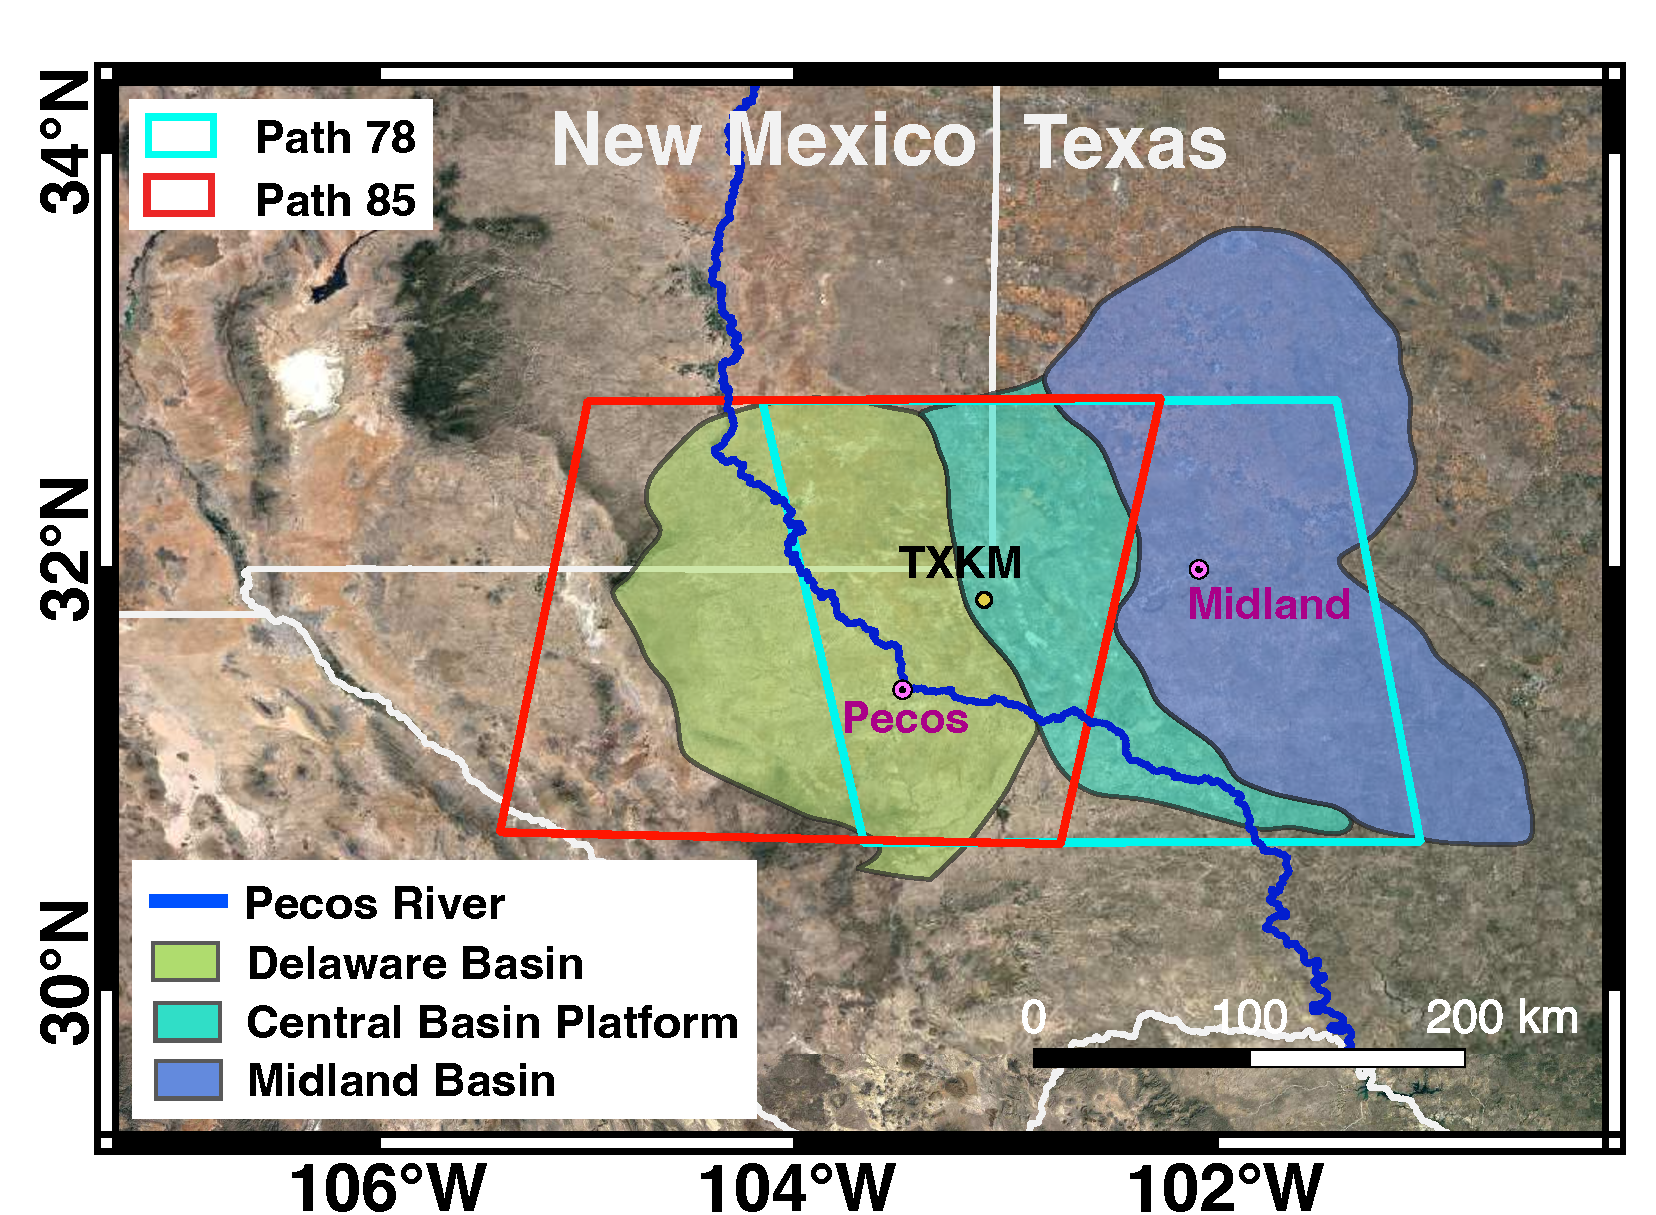
\includegraphics[width=0.9\linewidth]{figures/figure4-study-area.pdf}
	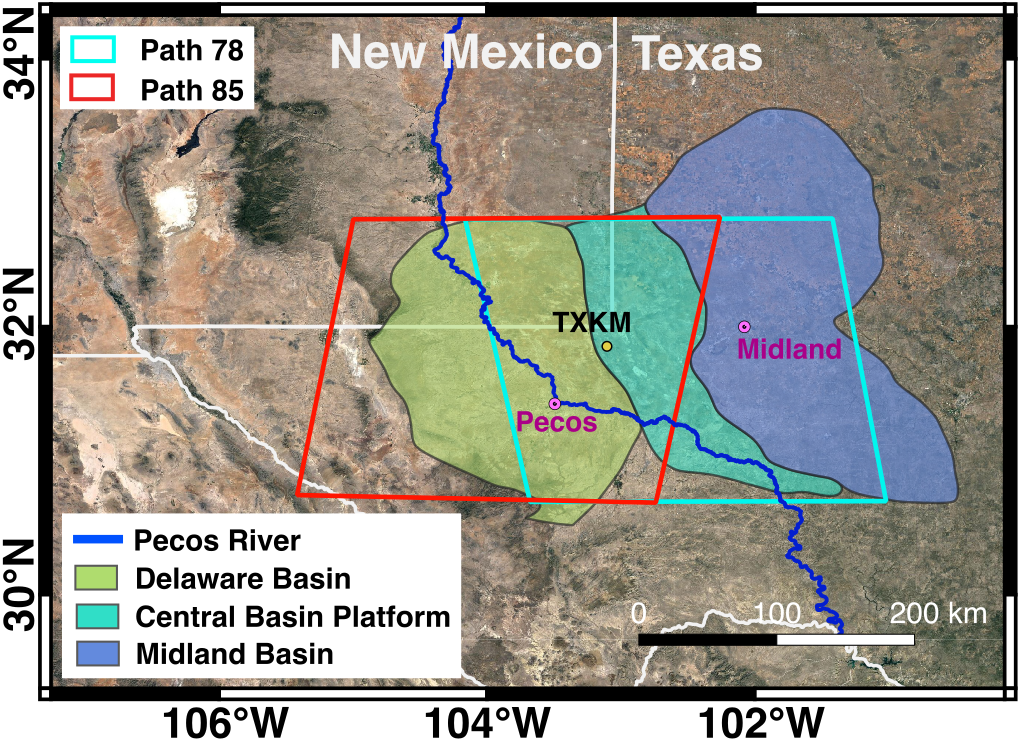
\includegraphics[width=0.96\linewidth]{paper2/figures/figure4-study-area.png}
	\caption[GPS and InSAR data coverage over the Permian Basin]{GPS and InSAR data coverage over the Permian Basin. Teal and red boxes indicate Sentinel-1 InSAR coverage for ascending Path 78 and descending Path 85. GPS station TXKM (yellow dot) was used as the reference point for both paths.
		%Each path contains over 80 SAR acquisitions, leading to over 3500 interferograms per path at 180 m pixel spacing.
	}
	\label{fig:study-area}
\end{figure}


We employed a stacking approach \citep{Sandwell1998PhaseGradientApproach, Staniewicz2020InsarRevealsComplex} to calculate the average LOS velocity $v_{avg}$ at each ground pixel over a time period of interest $ T $ as
\begin{equation}
	v_{avg} = \frac{\sum_{i \in G} d_i}{\sum_{i \in G} t_i}
	\label{eq:stacking-paper2}
\end{equation}
where $G$ is a subset of interferograms formed using two SAR scenes acquired within the time period $T$. The LOS measurement (in cm) and the temporal baseline of the $i^{th}$ interferogram in $G$ are written as $d_i$ and $ t_i $ respectively.
In this study, we used 29 SAR scenes acquired between November 2014 and January 2017 to solve for the average velocity during this period, and we computed the cumulative deformation as the average velocity times the total time span ($\sim 2$ years). Similarly, we used 52 SAR scenes acquired between November 2014 and January 2018, and 84 SAR scenes acquired between November 2014 to January 2019 to derive the cumulative deformation maps over these two study periods ($\sim 3$ and $4$ years).

We estimated the tropospheric turbulence noise for each SAR acquisition date using all interferograms that contain this SAR scene based on Equation \eqref{eq:avg-ifg}. We removed a quadratic ramp in each noise map, and calculated the average 1D PSD of all 84 noise maps as described in \ref{subsec:methods-2-tropo-spectrum}.
%The 800 day temporal baseline resulted in up to $\sim$80 interferograms per acquisition near the middle of the time period (which have 800 days available before and after the date).
Using the average noise spectrum, we generated 29 synthetic noise maps, which corresponds to the 29 Sentinel-1 acquisition dates between November 2014 and January 2017. We formed noise-only synthetic interferograms and calculated the cumulative stacking solution using Equation \eqref{eq:stacking-paper2}. We ran our blob detection algorithm on the noise-only stacking solution, and recorded the size, the filter response magnitude, and the magnitude of each noise blob feature. We repeated this process until the number of recorded detections exceeded 100,000. We smoothed the resulting histograms using a kernel density estimate (KDE) \citep{Scott2015MultivariateDensityEstimation}, and generated 2D empirical Probability Density Functions (PDFs) of the noise attributes for the November 2014-January 2018 cumulative LOS deformation map.
%We call this entire procedure one simulation, and we call the resulting set of detections one synthetic dataset. 
Similarly, we ran additional simulations to generate 2D histograms of the noise attributes for the November 2014-January 2018, and November 2014-January 2019 cumulative deformation maps.
%We repeated this simulation for the Nov. 2014 - Jan. 2018 time period using 52 simulated tropospheric turbulence maps, and for the Nov. 2014 - Jan. 2019 time period using 84 simulated tropospheric turbulence maps.
%we performed 3 rounds of simulation: one for the 2-year, 3-year, and 4-year cumulative deformation maps. For each round, we generated the same number of synthetic tropospheric turbulence noise maps as Sentinel-1 acquisitions.  
These histograms were then used to remove candidate blob features in the real Sentinel-1 InSAR deformation maps that are likely due to tropospheric noise artifacts.

We also processed 81 descending Sentinel-1 scenes (Path 85 Frames 483–493) acquired between November 2014 and January 2019 (Figure \ref{fig:study-area}). The same GPS station TXKM was used as the reference location to calibrate all interferograms. Following the same processing strategy, we estimated three cumulative deformation maps spanning November 2014 to January 2017, January 2018, and January 2019. We characterized the tropospheric noise from InSAR data, and identified deformation features in the cumulative deformation maps that are likely real.

\section{Results and Discussion}
\subsection{Path 78 detections}
\label{sec:results:path78}
%\subsection{Tropospheric Noise Power Spectra}
Figure \ref{fig:results-noise} (a)-(c) shows three estimated tropospheric noise maps for Sentinel-1 Path 78 acquisitions 2017-12-12, 2018-09-14, and 2017-06-15. We observe blob-like turbulence features ranging from a few kilometers up to tens of kilometers in diameter, and the magnitude of the tropospheric turbulence noise varies substantially on different days (Figure \ref{fig:results-noise} (d)). For example, the maximum absolute tropospheric noise observed on 2017-12-12, 2018-09-14, and 2017-06-15 are 1.8 cm, 3.2 cm, and 12.6 cm, respectively. Overall, $\sim$ 50\% of Path 78 scenes were acquired under quiet atmospheric conditions with a maximum noise level under 4 cm. Approximately, 35\% scenes were acquired under moderate turbulence conditions (a maximum noise level of 4-10 cm), and 15\% scenes were acquired under strong turbulent noise conditions (a maximum noise level of 11-15 cm). 

\begin{figure}
	\centering 
	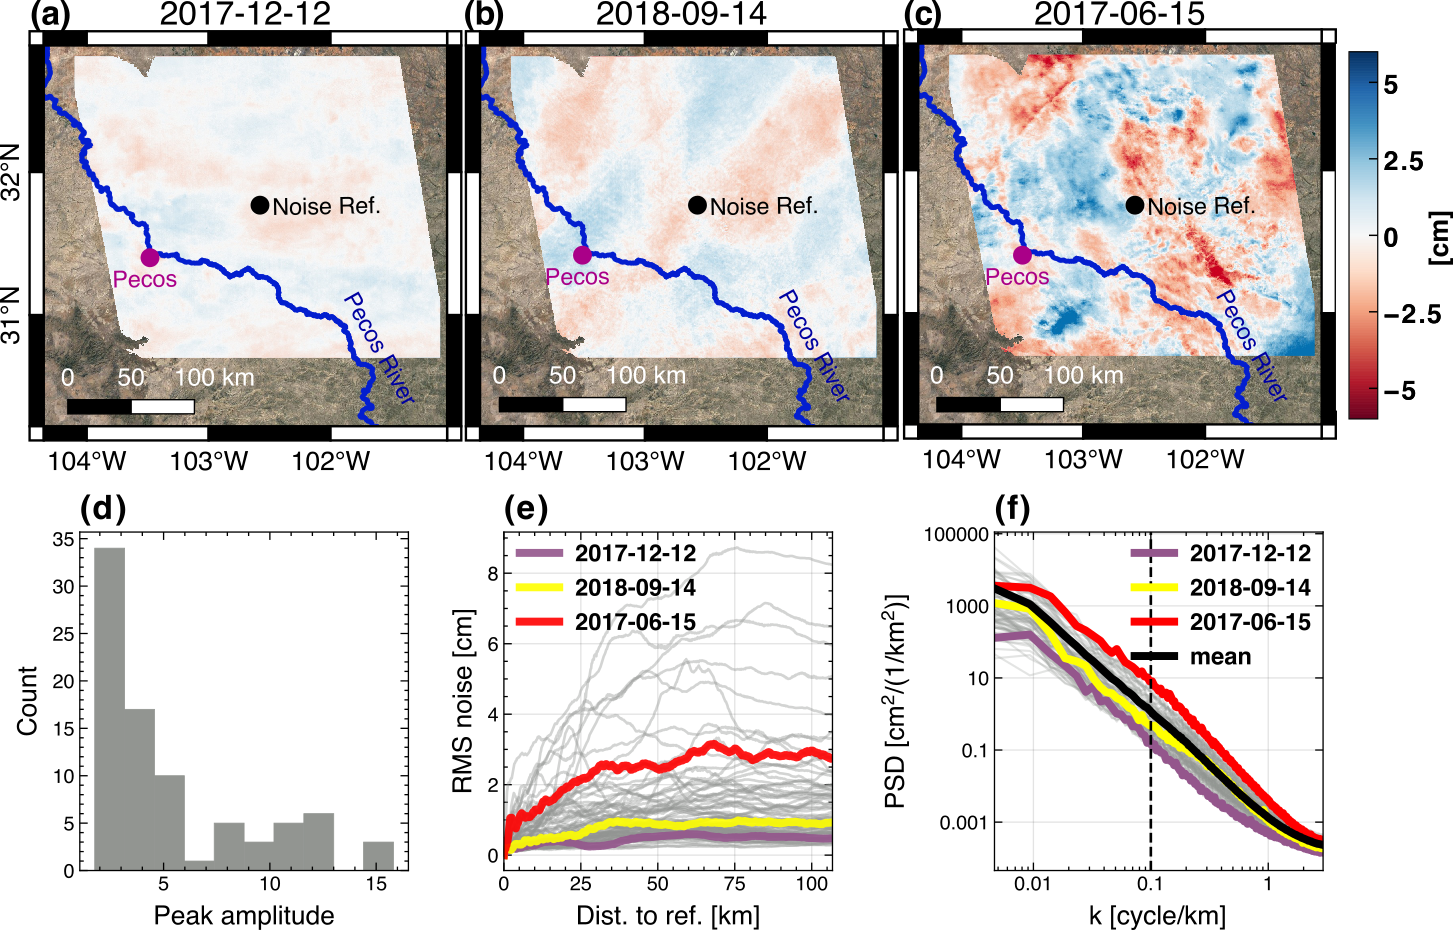
\includegraphics[width=.99\linewidth]{paper2/figures/figure5_noise_path78.png}
	%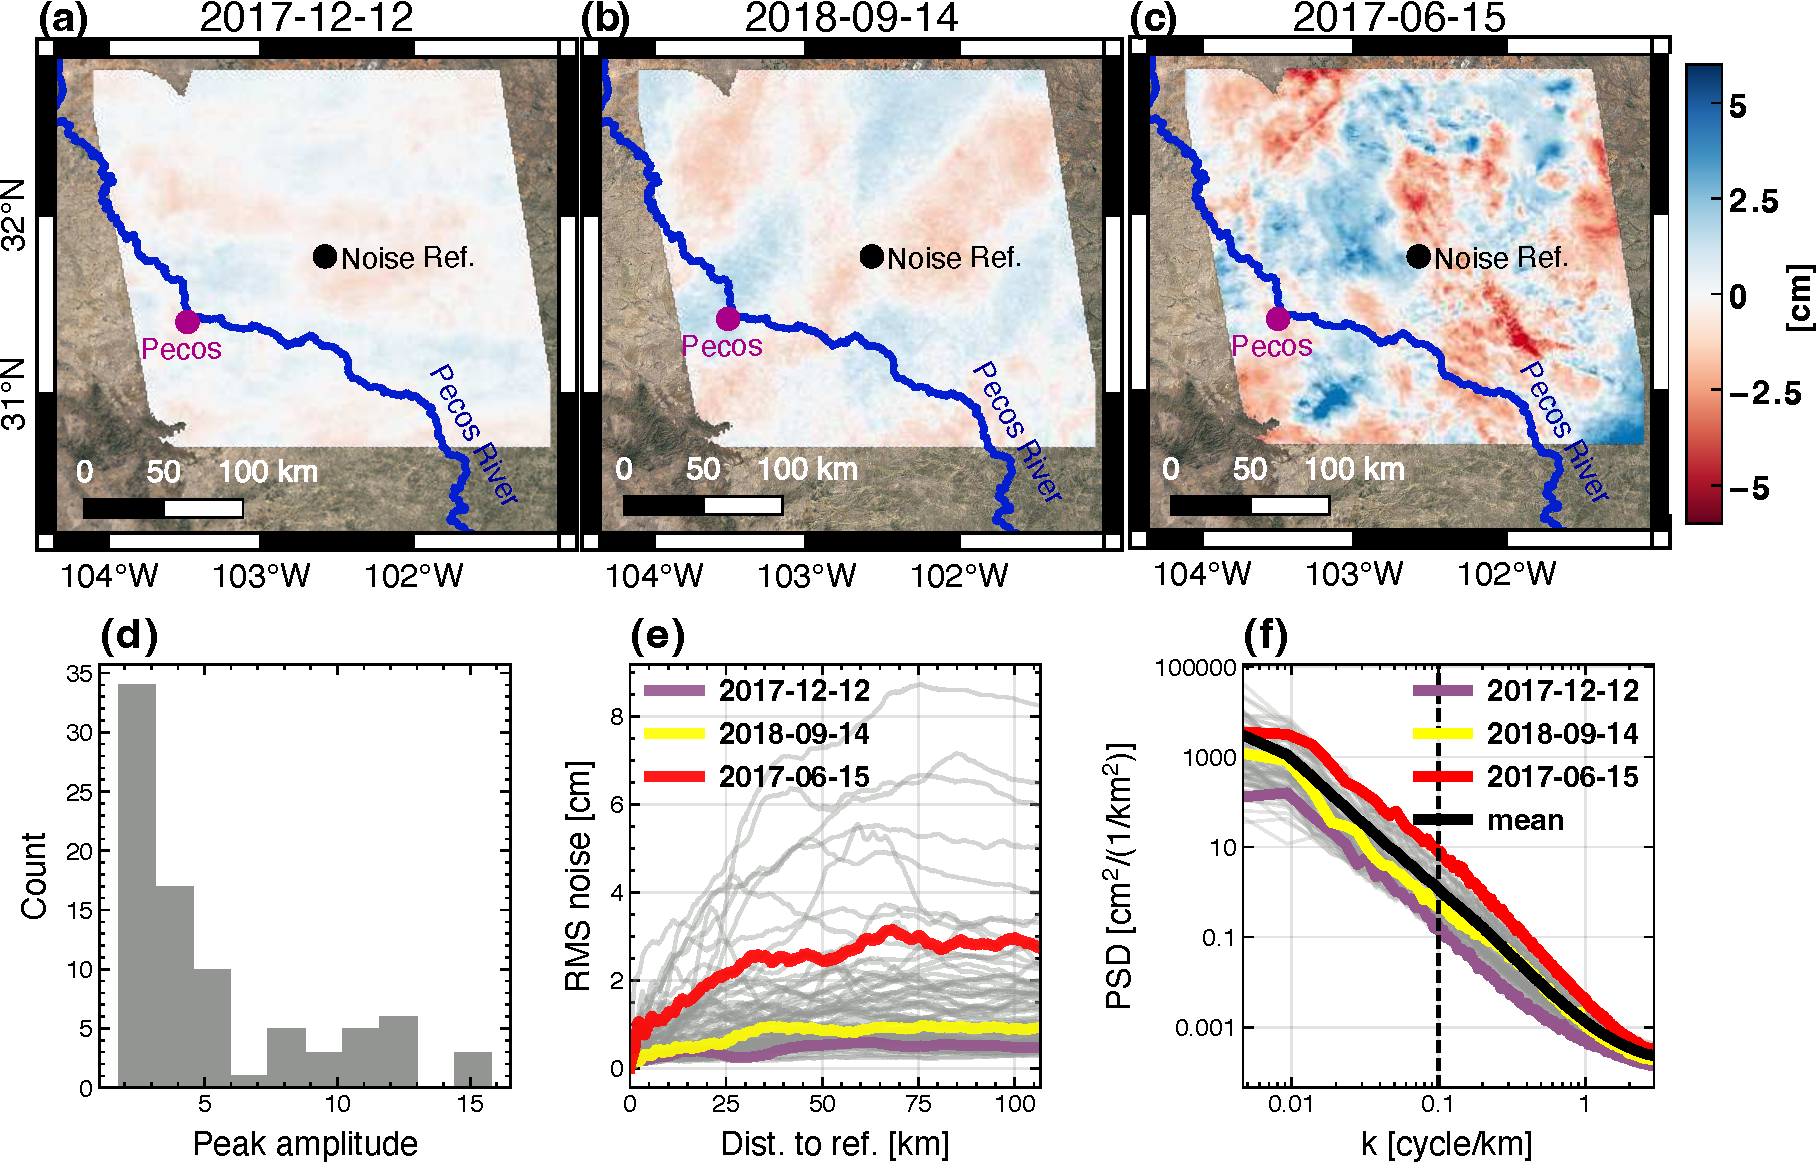
\includegraphics[width=0.98\linewidth]{figures/figure5_noise_path78.pdf}
	\caption[InSAR-estimated tropospheric turbulence noise maps for Path 78]{
		InSAR-estimated tropospheric turbulence noise maps for three Path 78 SAR acquisitions: (a) 2017-12-12 (up to 1.8 cm noise), (b) 2018-09-14 (up to 3.2 cm noise), and (c) 2017-06-15  (up to 12.6 cm noise).
		(d) The distribution of peak tropospheric noise magnitude (in centimeters), (e) the root mean squared value of tropospheric noise vs. distance from the center of the map, and (f) the estimated 1D PSDs for 84 Sentinel-1 Path 78 acquisitions used in this study. In panel (e) and (f), the color lines represent three SAR acquisitions (panel (a)-(c)) with different tropospheric noise levels. The black line in panel (f) represents the mean PSD of all 84 acquisitions.}
	\label{fig:results-noise}
\end{figure}


Because InSAR phases are measured with respect to a reference point, we calculated tropospheric noise estimates relative to the center of the map (the noise reference point). We plotted the mean absolute tropospheric noise vs. distance to the noise reference point (Figure \ref{fig:results-noise}(e)). For the majority of the Path 78 acquisitions, the turbulent noise increases as the square root of the distance for the first $\sim 50$ km, and then the magnitude of the tropopsheric noise does not change much as the distance increases. This means that the tropospheric noise is spatially correlated with a correlation length of $\sim 50$ km, and the tropospheric noise magnitude over the flat portion of the curve is a measure of the noise activity level. 

The 1D PSDs for the 84 tropospheric turbulence noise maps give an alternative view of the distribution of noise power over different frequencies (Figure \ref{fig:results-noise} (f). For most spatial frequencies, the PSDs decay following the -8/3 power law described in previous studies \citep{Hanssen2001RadarInterferometryData, Onn2006ModelingWaterVapor}. This slope flattens at the low frequencies because we removed the quadratic phase in the noise solutions. The slope also flattens at high frequencies, where decorrelation noise introduces pixel-level variations in the noise map.
%\subsection{Simulated tropospheric turbulence noise and Uncertainty Quantification}



\begin{figure}
	\centering 
	%\includegraphics[width=0.98\linewidth]{figures/figure_results_simulation_kde.png}
	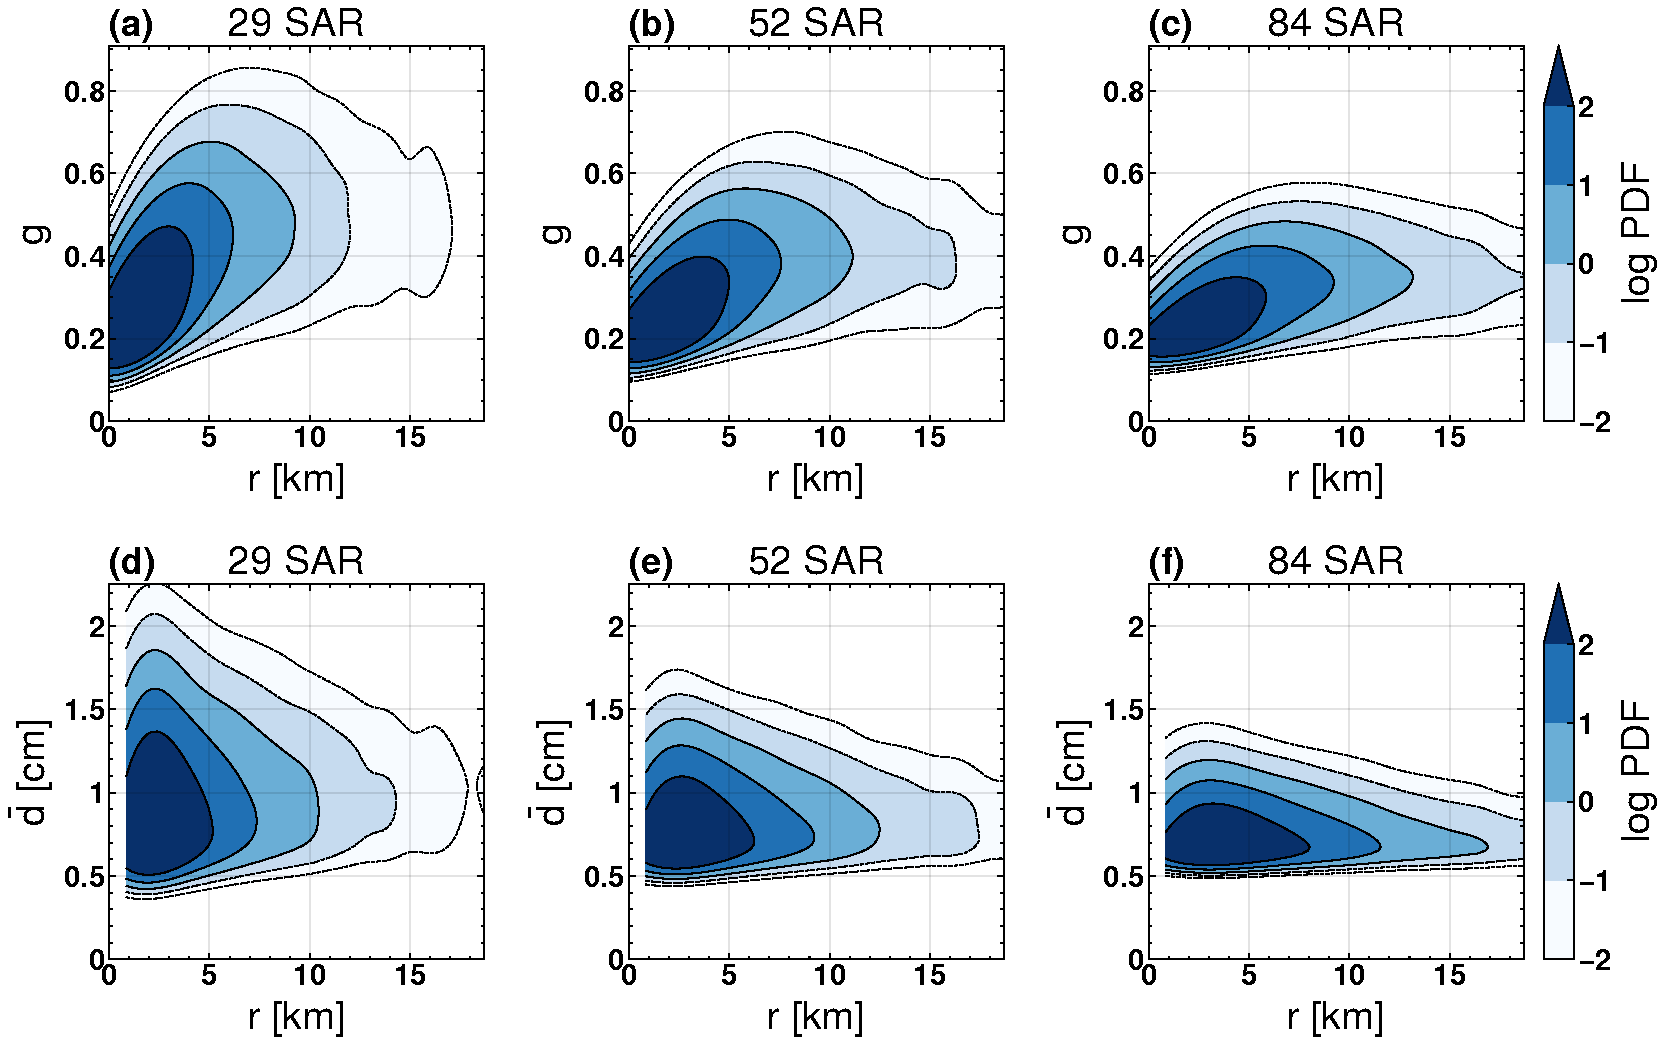
\includegraphics[width=0.98\linewidth]{paper2/figures/figure_results_kde.pdf}
	\caption[Estimates of empirical tropospheric noise probability density]{ (a)-(c) Log Probability Density Function (PDF) of detecting tropospheric noise blobs as a function of feature size $r$ and filter response magnitude $|g|$ for three cumulative LOS deformation maps: November 2014 - January 2017 (29 SAR scenes from Path 78), November 2014 - January 2018 (52 SAR Scenes from Path 78), and November 2014 - January 2019 (84 SAR Scenes from Path 78).
		(d)-(f) Log Probability Density Function (PDF) of detecting tropospheric noise blobs as a function of feature size $r$ and deformation magnitude $|d|$ for the same three cumulative LOS deformation maps.
		Here the PDFs were generated from 2D histograms using a kernel density estimate (KDE) \citep{Scott2015MultivariateDensityEstimation}.
	}
	\label{fig:results-kde}
\end{figure}



Using the mean 1D PSD shown in Figure \ref{fig:results-noise} (f), we simulated instances of tropospheric turbulence, and computed the empirical PDFs of the noise attributes for each deformation map (Figure \ref{fig:results-kde}).  Most of detected noise features have small radii ($r <$ 5 km). For the 29 SAR acquisition case, the noise features are unlikely to be larger 2 cm in magnitude or have a filter response stronger than 0.7 (Figure \ref{fig:results-kde} (a), (d)). For the 52 SAR acquisition case, the noise features are unlikely to be larger 1.5 cm in magnitude or have a filter response stronger than 0.6 (Figure \ref{fig:results-kde} (b), (e)). For the 84 SAR acquisition case, the noise features are unlikely to be larger 1.2 cm in magnitude or have a filter response stronger than 0.5 (Figure \ref{fig:results-kde} (c), (f)).
%(Figure \ref{fig:results-kde}(a-c)). The noise instances are spatially isotropic and contain many $\sim$3 cm blob-like features ranging from several km up to $\sim$100 km in length. As outlined in Section \ref{sec:site}, we computed three LOS deformation maps from 29,52, and 84 noise instances, and we recorded all detected noise features. The resulting histograms of ($g$ vs. $r$ and $\bar{d}$ vs. $r$) were smoothed using a kernel density estimate (KDE) \citep{Scott2015MultivariateDensityEstimation} to create 2D empirical probability density functions (PDFs) (Figure \ref{fig:results-kde}). As the number of SAR acquisitions increases to 52 (Figure \ref{fig:results-kde}(b),(e)) and 84 (Figure \ref{fig:results-kde}(c),(f)), the amplitudes of detected noise features decreases for all $r$.
Note that the maximum and minimum sizes of detected features in Figure \ref{fig:results-kde} (d)-(f) are determined by the choice of maximum and minimum kernel sizes $\sigma_{max}$ and $\sigma_{max}$ in our automatic detection algorithm. By imposing the prior knowledge that oil and gas-production related deformation bowls are unlikely to be larger than 30-40 km in the Permian Basin \citep{Staniewicz2020InsarRevealsComplex}, $\sigma_{max}$ was set so that the maximum detected feature radius $r$ was approximately 20 km. Thus, large-scale tropospheric noise features ($>$ 20 km) were not recorded in the noise simulations.
%\subsection{West Texas Detected Deformation}




Using the empirical PDFs of the noise attributes, we removed detections with more than 5\% chance of being noise from three Path 78 cumulative deformation maps (Figure \ref{fig:results-detections}). We identified 57 remaining deformation features in the Nov. 2014-Jan. 2017 cumulative deformation map, 147 features in the Nov. 2014-Jan. 2018 map, and 268 features in the Nov. 2014-Jan. 2019 map. The increasing number of detected deformation features is due to (1) the oil and gas production rate experienced a sharp rise over the study period \citep{Staniewicz2020InsarRevealsComplex}; and (2) a larger number of SAR acquisitions reduces the noise level in the InSAR cumulative deformation solutions.

\begin{figure}
	\centering 
	%\includegraphics[width=0.98\linewidth]{figures/figure_results_detections_vert.png}
	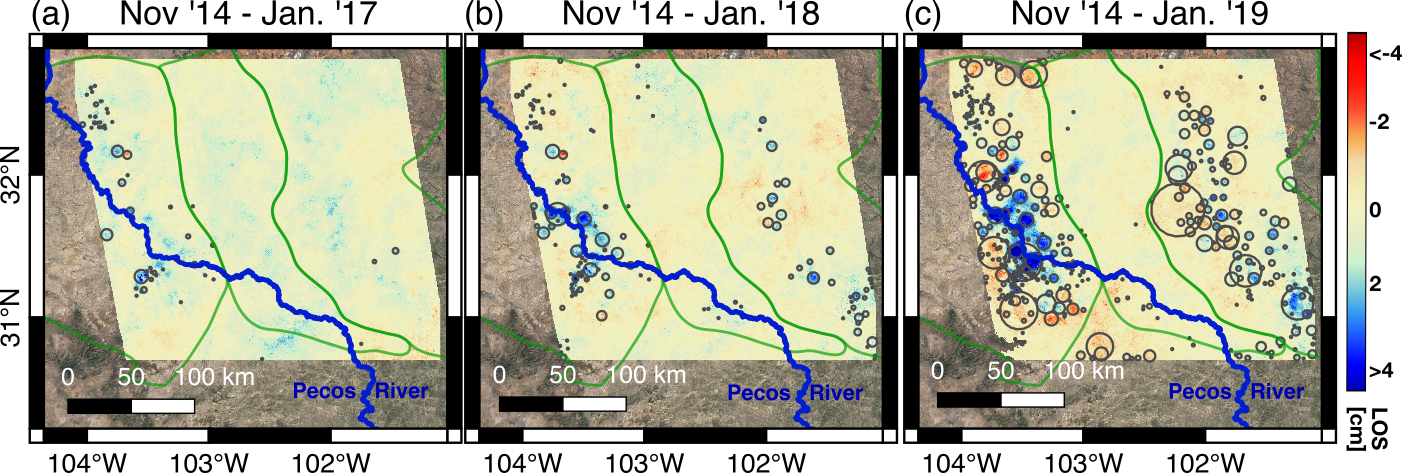
\includegraphics[width=0.98\linewidth]{paper2/figures/figure_results_blobs_path78.png}
	\caption[Detected deformation figures from the three Path 78 cumulative LOS deformation maps]{
		Detected deformation features (gray circles) from the three Path 78 cumulative LOS deformation maps. Features with more than 5\% chance of being noise for their radius, according to either the filter magnitude or image magnitude PDFs (Figure \ref{fig:results-kde}), have been removed. Green lines correspond the boundaries of the Delaware Basin, Central Basin Platform, and Midland Basin from west to east.
		% Not shown are features which, given their radius, have with more than 5\% chance of being noise according to either the filter magnitude or image magnitude PDFs (Figure \ref{fig:results-kde}). 
	}
	\label{fig:results-detections}
\end{figure}






The detected features are mainly clustered in regions within the Midland Basin and the Delaware Basin. Here oil production and wasterwater injection caused many centimeter-level subsidence and uplift features. In the Southern Delaware Basin, the observed linear deformation features parallel the inferred favorable fault plane orientation proposed by \cite{LundSnee2018StateStressPermian}, and they align with a cluster of recent shallow earthquakes cataloged by TexNet. Very few deformation features were detected in the Central Basin Platform, where oil and gas are mostly produced from conventional reservoirs and the subsurface pressure was well maintained.

For the West Texas case, the residual deformation term $  \frac{1}{N-1}  \sum  \Delta d_{n,k} $ in Equation \eqref{eq:avg-ifg} does not significantly influence our noise simulations. To demonstrate this, Figure \ref{fig:discussion-residual-defo} (a) shows the tropospheric noise estimates on a quiet atmospheric date (2018-09-04) and Figure  \ref{fig:discussion-residual-defo} (b) shows the cumulative LOS deformation solution between  Nov. 2014 and Jan. 2019. The 1D PSDs for the noise-only map and the noise plus deformation map are very similar (Figure \ref{fig:discussion-residual-defo} (c)). This is because the total integrated power of the noise map is 3.5 cm$^2 $, five times larger than the total power of the deformation map (0.7 cm$^2 $). Since the residual deformation contribution in Equation \eqref{eq:avg-ifg}, $ \frac{1}{N-1}  \sum  \Delta d_{n,k} $, is much less than the total cumulative deformation over the entire study period, we conclude that this term in the tropospheric noise estimates has negligible effects on the ultimate detection confidences resulting from the simulations.


\begin{figure}[hbt!]
	\centering 
	% vertical version:
	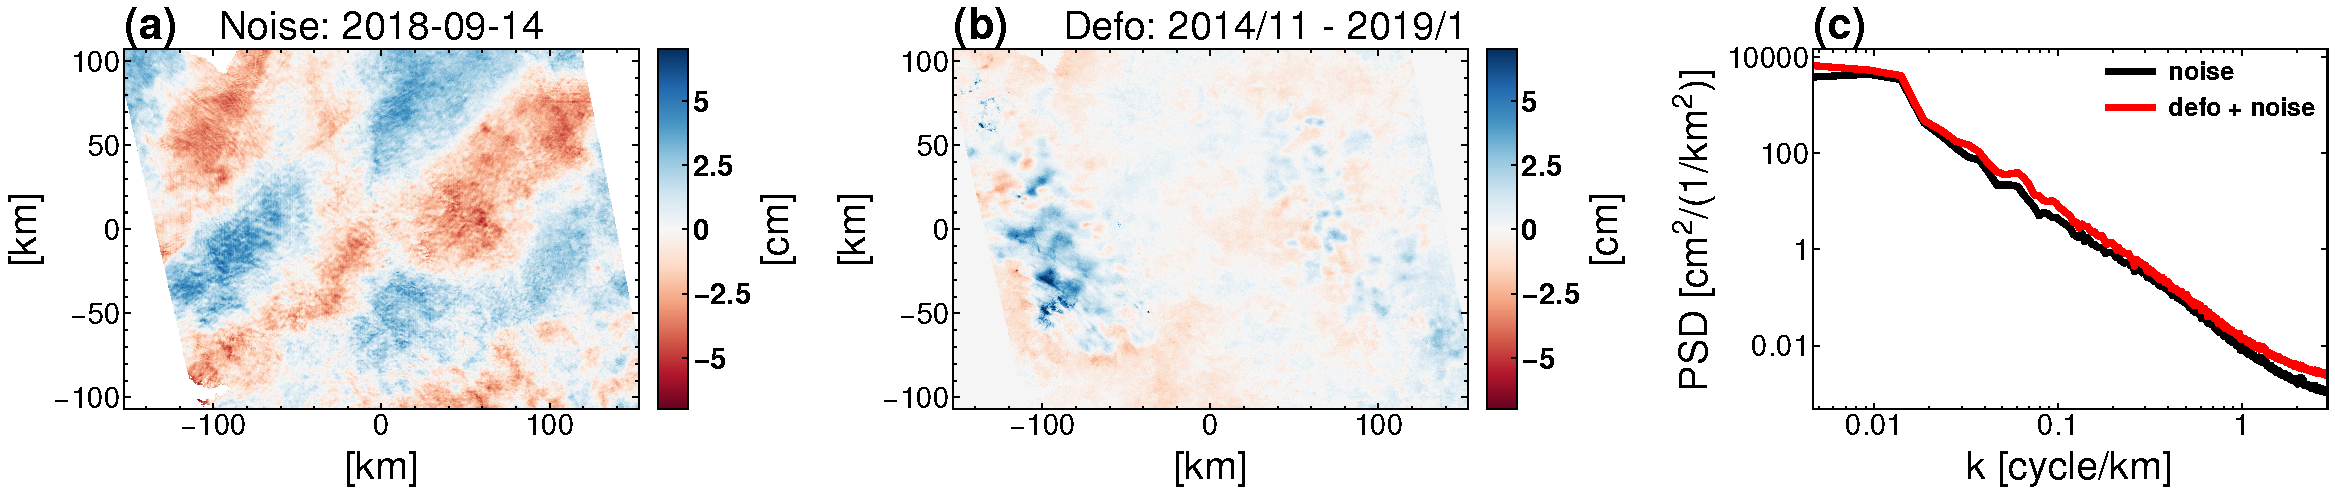
\includegraphics[width=0.98\linewidth]{paper2/figures/figure_discussion_residual_defo.pdf}
	%\includegraphics[width=0.98\linewidth]{figures/figure_discussion_residual_defo_horizontal.pdf}
	\caption[Effect of residual deformation on tropospheric PSD estimate]{
		(a) InSAR-estimated tropospheric noise map for the Path 78 SAR acquisition 2018-09-14. 
		(b) Cumulative LOS deformation from Nov. 2014 to Jan. 2019 as inferred from Sentinel-1 Path 78 InSAR data.
		(c) 1D PSDs derived from the tropospheric noise map (black) and the tropospheric noise plus deformation map (red).
	}
	\label{fig:discussion-residual-defo}
\end{figure}


\subsection{Path 85 Detections}
\label{subsec:discussion-path85}

Due to the differences in acquisition times (7:50 p.m. local time for path 78, 6:55 a.m. for path 85), the turbulence is milder on average for path 85 (Figure \ref{fig:discussion-noise-85}). Similar to path 78 (shown in Figure \ref{fig:results-noise}(d)), approximately 50\% of SAR acquisitions have quiet atmospheric conditions with a peak noise level under 4 cm (Figure \ref{fig:discussion-noise-85}a). However, there are only two path 85 acquisitions with over 10 cm of peak noise, compared to 14 acquisitions for path 78. The difference in noise level is also apparent in the growth of RMS noise vs. distance to the reference point (Figure \ref{fig:discussion-noise-85}b). While the shape of the growth is similar for ascending and descending, the ascending path 78 has 50\% larger average noise at 50 km from the reference. Similarly, the average PSDs for path 78 and path 85 have similar shape (Figure \ref{fig:discussion-noise-85}b), but the mean power for path 78 is over 2 times larger at a spatial frequency of 0.1 cycles/km. We summarized the noise statistical differences by comparing 1) the mean variance of each noise map, 2) the largest variance of any map, 3) the mean peak amplitude of the noise map, and 4) the largest peak across all dates (Table \ref{tab:path85-compare}).


\begin{figure}[hbt!]
	\centering 
	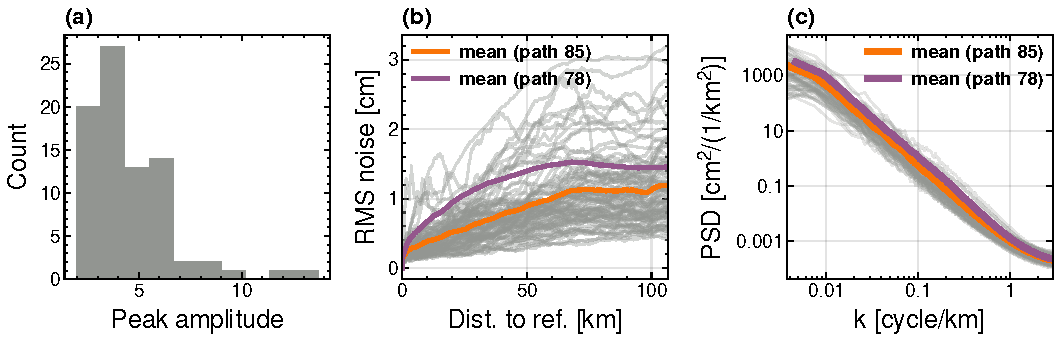
\includegraphics[width=0.98\linewidth]{paper2/figures/figure_discussion_path85_plots.pdf}
	\caption[Estimated tropospheric noise for Sentinel-1 Path 85]{(a) The distribution of peak tropospheric noise magnitude (in centimeters), (b) the root mean squared value of tropospheric noise vs. distance from the center of the map, and (c) the estimated 1D PSDs for 81 Sentinel-1 Path 85 acquisitions used in this study. In panel (b) and (c), the color lines represent the average estimates for Path 85 (orange) and Path 78 (purple).
	}
	\label{fig:discussion-noise-85}
\end{figure}




\begin{table}
	\centering
	\caption{Tropospheric noise characteristics for Sentinel-1 Path 85 and Path 78 data over West Texas}
	\begin{tabular}{lrr}
		\toprule
		{} &  Path 78 &  Path 85 \\
		\midrule
		Average Variance [cm$^2$]             &     1.38 &     0.78 \\
		Variance of Noisiest Date [cm$^2$] &    10.68 &     3.74 \\
		Average Peak Amplitude [cm]            &     5.36 &     4.58 \\
		Largest Peak Amplitude [cm]         &    15.81 &    13.72 \\
		%\midrule
		%Detected features with confidence $p<0.05$ & & \\
		%\midrule
		%Through Jan '17 & 48 & 58 \\
		%Through Jan '18 & 102 & 130 \\
		%Through Jan '19 & 256 & 343 \\
		\bottomrule
	\end{tabular}
	\label{tab:path85-compare}
\end{table}


Due to the weaker noise of path 85, there are more detected features at a confidence level of p $< 0.05 $ (Figure \ref{fig:discussion-detections-85}). Our algorithm found similar numbers of total deformation candidates in path 78 and path 85 (between 1000-1500 per year); most of these candidates are faint noise artifacts and given a low confidence score. However, the same feature detected in path 85 and path 78 has a higher confidence score in path 85 due to the lower average noise. While both path 78 and path 85 detect with high confidence the significant deformation in the Delaware Basin, there are several $\sim1$cm uplift bowls near wastewater injection wells in the Central Basin Platform which only pass the 95\% confidence threshold in path 85. 

\begin{figure}[hbt!]
	\centering 
	%\includegraphics[width=0.98\linewidth]{figures/figure_discussion_blobs_path85.png}
	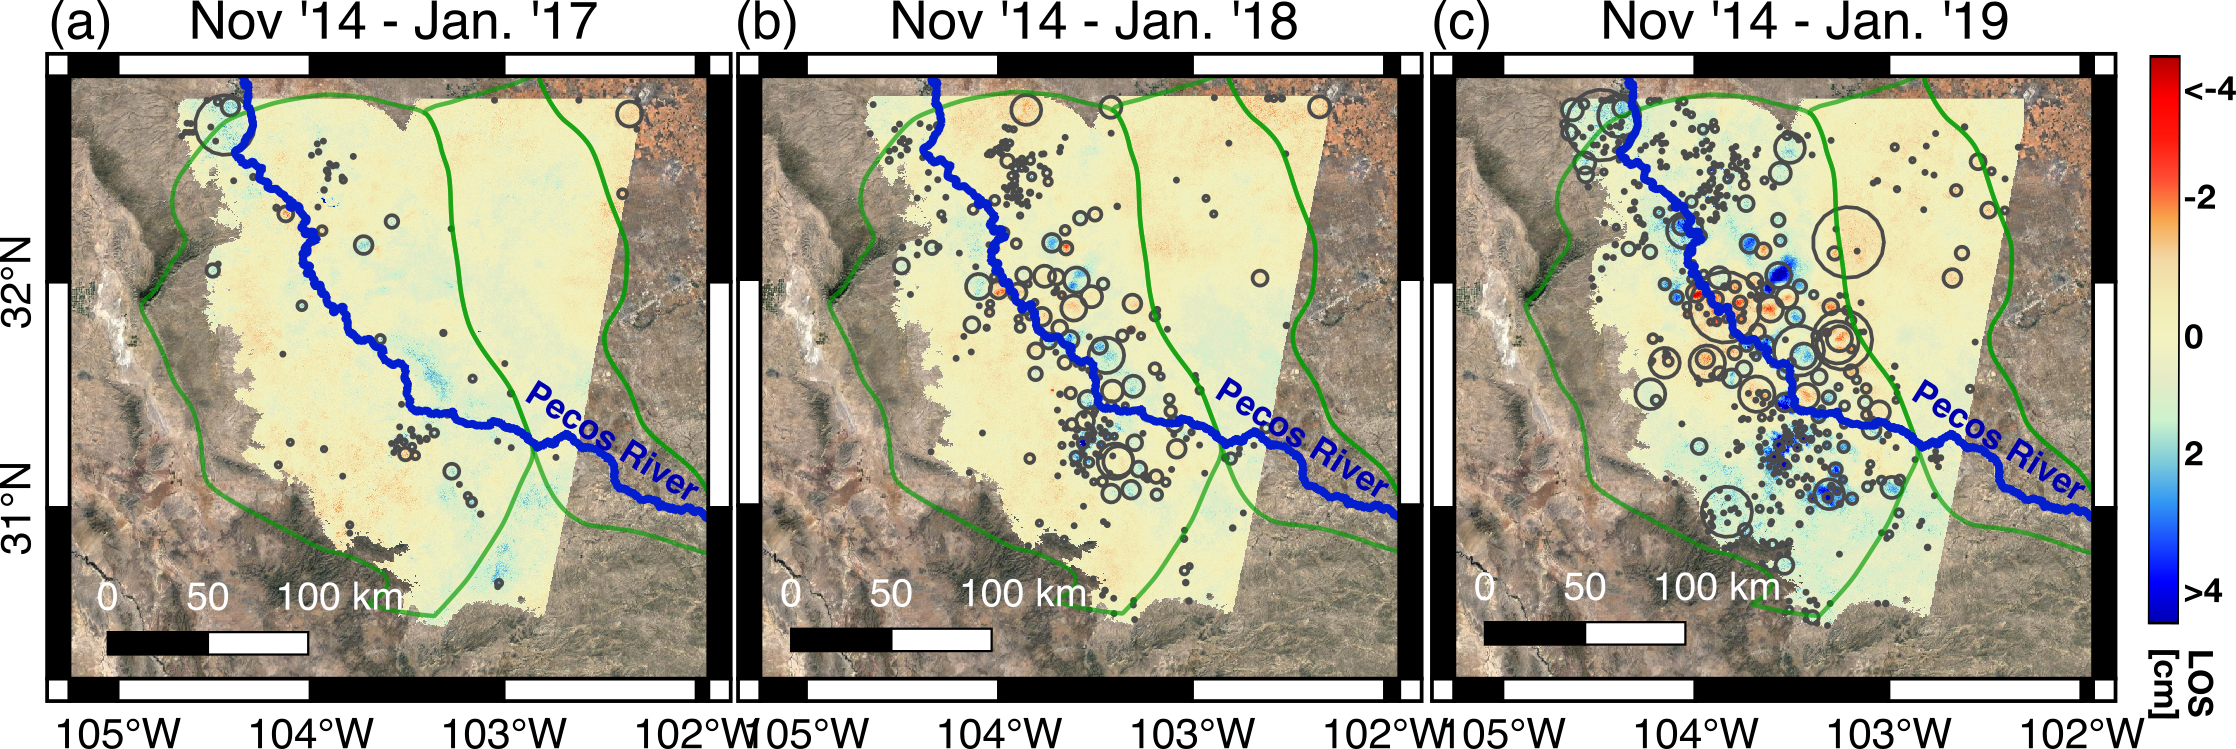
\includegraphics[width=0.98\linewidth]{paper2/figures/figure_discussion_blobs_combined_path85.png}
	\caption[Detected deformation features from the three Path 85 cumulative LOS deformation maps]{
		Detected deformation features (gray circles) from the three Path 85 cumulative LOS deformation maps. Features with more than 5\% chance of being noise for their radius, according to either the filter magnitude or image magnitude PDFs (Figure \ref{fig:results-kde}), have been removed. Green lines illustrate the boundaries of the Delaware Basin and Central Basin Platform, from west to east.
		%The blobs with more than 5\% chance to be noise, given their radius within the filter magnitude and image magnitude PDFs
	}
	\label{fig:discussion-detections-85}
\end{figure}



It is also worth noting that both paths show a large increase in the number of detections from 2016 though the end of 2018, coinciding with the overall rise in oil production within the Permian Basin (Figure \ref{fig:discussion-oil-blob-count}). While some of the increase in high confidence detections is due to the availability of more SAR acquisitions, the total oil production in the Permian Basin increased $>60\%$, from an average daily production of 1.5 Mbbl / day in 2016 to 2.5 Mbbl / day in 2018. This led to a large number of subsidence and uplift bowls detected in the Midland and Delaware Basins.

\begin{figure}[hbt!]
	\centering 
	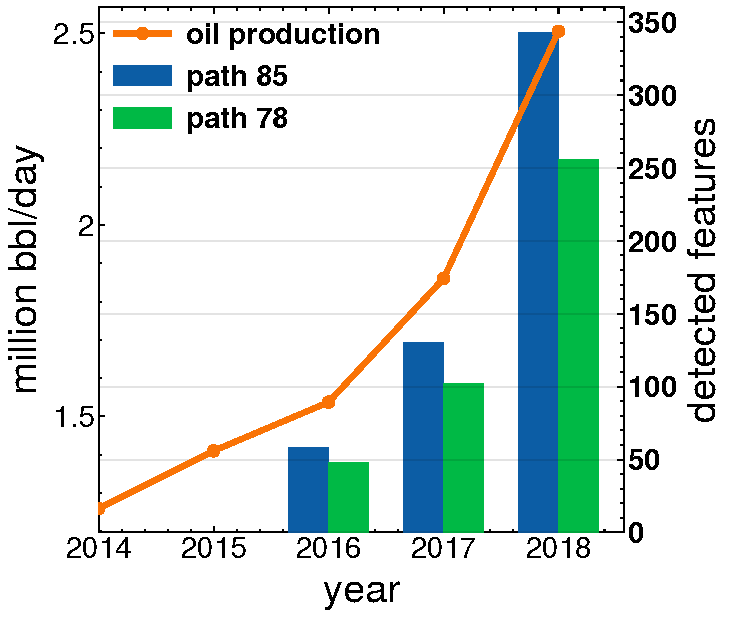
\includegraphics[width=0.98\linewidth]{paper2/figures/figure_discussion_oil_vs_blob_count.pdf}
	\caption[Number of detected deformation figures and yearly oil production]{
		The number of deformation features ($<$ 5\% of being tropospheric noise) detected from three Path 78 cumulative LOS deformation maps (Figure \ref{fig:results-detections}) and three Path 85 cumulative LOS deformation maps (Figure \ref{fig:discussion-detections-85}). Only detections from the overlapping region of the two paths are countered. The Permian Basin average daily oil production from 2014 and 2018 is shown as the orange line.
	}
	\label{fig:discussion-oil-blob-count}
\end{figure}



\section{Conclusion}


In this study, we developed a computer vision algorithm for automatically detecting the size and location of deformation features in InSAR maps. We characterized the tropospheric noise signatures directly from InSAR data, and removed false positive detections that are likely associated with  tropospheric artifacts. Our algorithm does not require labeled training data, and it can be integrated to existing InSAR time series methods to identify deformation features with different characteristics. This study demonstrates how computer vision algorithms can be used for large-scale InSAR data analysis and uncertainty quantification.


	
